% !TeX spellcheck = cs_CZ
%{\tikzset{external/prefix={tikz/FYZII/}}
% \tikzset{external/figure name/.add={ch23_}{}}
%---------------------------------------------------------------------------------------------------
% file fey2ch23.tex
%---------------------------------------------------------------------------------------------------
%====================Kapitola: Dutinové rezonátory =================================================
\setchaptertoc
\chapter{Dutinové rezonátory}\label{fyz:IIchapXXIII}

\section{Reálné prvky obvodů}\label{fyz:IIchapXXIIIsecI}
\section{Kondenzátor při vysokch frekvencích}\label{fyz:IIchapXXIIIsecII}
\section{Rezonanční dutina}\label{fyz:IIchapXXIIIsecIII}
\section{Kmitavé mody dutinových rezonátorů}\label{fyz:IIchapXXIIIsecIV}
\section{Dutinové rezonátory a rezonanční obvody}\label{fyz:IIchapXXIIIsecV}

    \begin{figure}[ht!] %\ref{fyz:fig583}
      \centering
      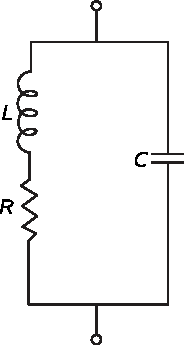
\includegraphics[width=0.3\linewidth]{fyz_fig583.pdf}
      \caption{
               (\cite[s.~707]{Feynman02})}
      \label{fyz:fig583}
    \end{figure}

    \begin{figure}[ht!]
      \centering
      \subcaptionbox{\label{fyz:fig584a}}{\luafigure[0.3]{fyz_fig584a.pdf}}
      \subcaptionbox{\label{fyz:fig584b}}{\luafigure[0.3]{fyz_fig584b.pdf}}
      \caption{
               (\cite[s.~748]{Feynman02})}
      \label{fyz:fig584}
    \end{figure}

    pokus \ref{fyz:fig584} nebo \ref{fyz:fig584b}
    
    \begin{figure}[ht!]
      \centering
      \subcaptionbox{\label{fyz:fig585a}}{\luafigure[0.3]{fyz_fig585a.pdf}}
      \subcaptionbox{\label{fyz:fig585b}}{\luafigure[0.3]{fyz_fig585b.pdf}}
      \subcaptionbox{\label{fyz:fig585c}}{\luafigure[0.3]{fyz_fig585c.pdf}}
      \label{fyz:fig585}
      \caption{
               (\cite[s.~748]{Feynman02})}
    \end{figure}

    \begin{figure}[ht!] %\ref{fyz:fig586}
      \centering
      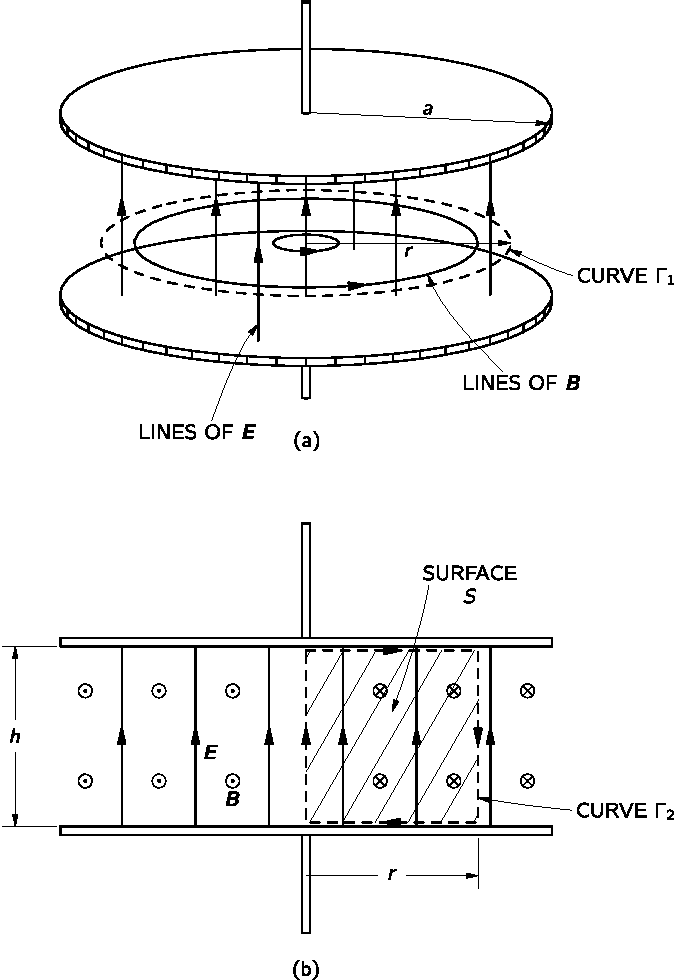
\includegraphics[width=0.7\linewidth]{fyz_fig586.pdf}
      \caption{
               (\cite[s.~707]{Feynman02})}
      \label{fyz:fig586}
    \end{figure}
    
    \begin{figure}[ht!] %\ref{fyz:fig587}
      \centering
      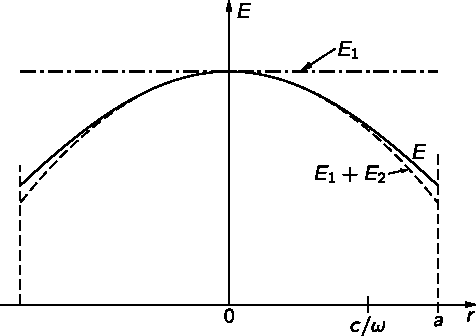
\includegraphics[width=0.7\linewidth]{fyz_fig587.pdf}
      \caption{
               (\cite[s.~707]{Feynman02})}
      \label{fyz:fig587}
    \end{figure}

    \begin{figure}[ht!] %\ref{fyz:fig588}
      \centering
      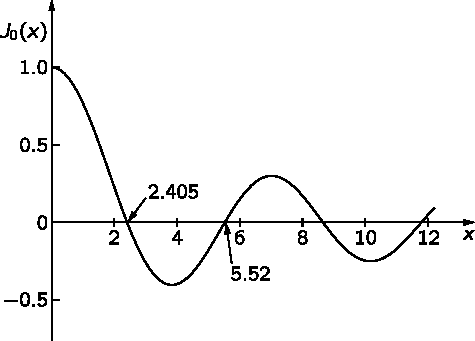
\includegraphics[width=0.7\linewidth]{fyz_fig588.pdf}
      \caption{
               (\cite[s.~707]{Feynman02})}
      \label{fyz:fig588}
    \end{figure}

    \begin{figure}[ht!]
      \centering
      \subcaptionbox{\label{fyz:fig589a}}{\luafigure[0.7]{fyz_fig589a.pdf}}               \\
      \subcaptionbox{\label{fyz:fig589b}}{\luafigure[0.7]{fyz_fig589b.pdf}}              
      \caption{Pohyb tekutiny v proudové trubici
               (\cite[s.~748]{Feynman02})}
    \end{figure}

    \begin{figure}[ht!] %\ref{fyz:fig590}
      \centering
      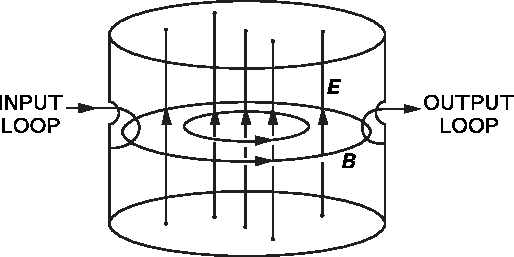
\includegraphics[width=0.7\linewidth]{fyz_fig590.pdf}
      \caption{
               (\cite[s.~707]{Feynman02})}
      \label{fyz:fig590}
    \end{figure}
    
    \begin{figure}[ht!] %\ref{fyz:fig591}
      \centering
      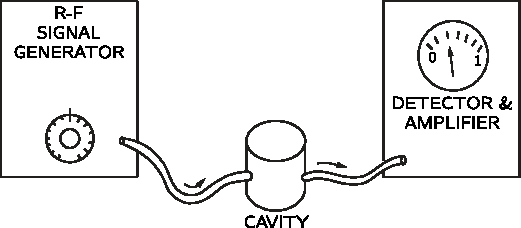
\includegraphics[width=0.7\linewidth]{fyz_fig591.pdf}
      \caption{
               (\cite[s.~707]{Feynman02})}
      \label{fyz:fig591}
    \end{figure}

    \begin{figure}[ht!] %\ref{fyz:fig592}
      \centering
      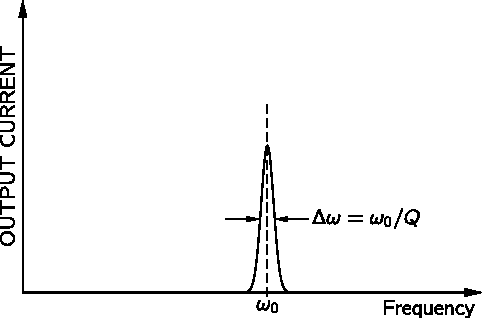
\includegraphics[width=0.7\linewidth]{fyz_fig592.pdf}
      \caption{
               (\cite[s.~707]{Feynman02})}
      \label{fyz:fig592}
    \end{figure}

    \begin{figure}[ht!] %\ref{fyz:fig593}
      \centering
      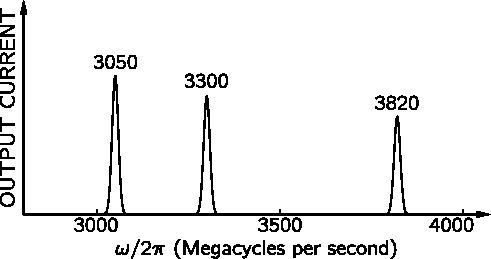
\includegraphics[width=0.7\linewidth]{fyz_fig593.pdf}
      \caption{
               (\cite[s.~707]{Feynman02})}
      \label{fyz:fig593}
    \end{figure}

    \begin{figure}[ht!]
      \centering
      \subcaptionbox{\label{fyz:fig594a}}{\luafigure[0.5]{fyz_fig594a.pdf}}               \\
      \subcaptionbox{\label{fyz:fig594b}}{\luafigure[0.5]{fyz_fig594b.pdf}}              
      \caption{
               (\cite[s.~748]{Feynman02})}
    \end{figure}

    \begin{figure}[ht!] %\ref{fyz:fig595}
      \centering
      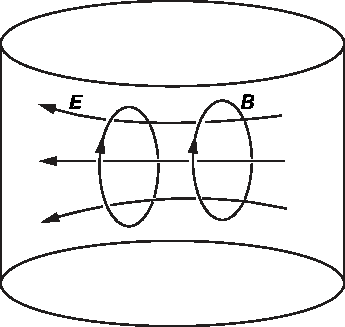
\includegraphics[width=0.5\linewidth]{fyz_fig595.pdf}
      \caption{
               (\cite[s.~707]{Feynman02})}
      \label{fyz:fig595}
    \end{figure}

    \begin{figure}[ht!] %\ref{fyz:fig596}
      \centering
      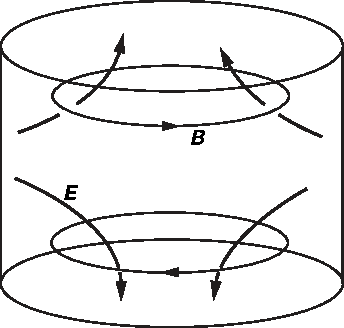
\includegraphics[width=0.5\linewidth]{fyz_fig596.pdf}
      \caption{
               (\cite[s.~707]{Feynman02})}
      \label{fyz:fig596}
    \end{figure}

    \begin{figure}[ht!]
      \centering
      \subcaptionbox{\label{fyz:fig597a}}{\luafigure[0.45]{fyz_fig597a.pdf}}
      \subcaptionbox{\label{fyz:fig597b}}{\luafigure[0.45]{fyz_fig597b.pdf}}               \\
      \subcaptionbox{\label{fyz:fig597c}}{\luafigure[0.45]{fyz_fig597c.pdf}}
      \caption{
               (\cite[s.~748]{Feynman02})}
      \label{fyz:fig597}
    \end{figure}

    \begin{figure}[ht!]
      \centering
      \subcaptionbox{\label{fyz:fig598a}}{\luafigure[0.6]{fyz_fig598a.pdf}}               \\
      \subcaptionbox{\label{fyz:fig598b}}{\luafigure[0.6]{fyz_fig598b.pdf}}               \\
      \subcaptionbox{\label{fyz:fig598c}}{\luafigure[0.7]{fyz_fig598c.pdf}}
      \caption{
               (\cite[s.~748]{Feynman02})}
      \label{fyz:fig598}
    \end{figure}

    \begin{figure}[ht!] %\ref{fyz:fig599}
      \centering
      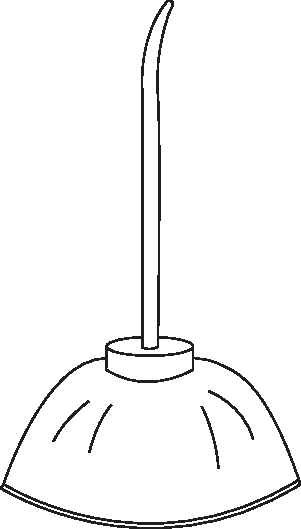
\includegraphics[width=0.3\linewidth]{fyz_fig599.pdf}
      \caption{
               (\cite[s.~707]{Feynman02})}
      \label{fyz:fig599}
    \end{figure}

    \todo[inline]{Kapitola fey2ch23 je nedodělaná, obsahuje pouze obrázky}
%} %tikzset
%~~~~~~~~~~~~~~~~~~~~~~~~~~~~~~~~~~~~~~~~~~~~~~~~~~~~~~~~~~~~~~~~~~~~~~~~~~~~~~~~~~~~~~~~~~~~~~~~~~
